\documentclass[english]{beamer} %,handout
\usepackage{amsmath}
\usepackage{graphicx}
\usepackage[cjk,hangul,usecjkt1font]{kotex}

\makeatletter

\usepackage{listings}
\setbeamertemplate{footline}[frame number]
\setbeamercovered{transparent}

\usecolortheme{kesl}

\usepackage[absolute,overlay]{textpos}
\setlength{\TPHorizModule}{\paperwidth}
\setlength{\TPVertModule}{\paperheight}
\textblockorigin{0mm}{0mm}
 
\usepackage{babel}
\beamertemplatenavigationsymbolsempty
\usepackage{verbatim}
\begin{document}

\title[Memory Scalability]{
경량 로그 기반 지연 업데이트 기법을 활용한 리눅스 커널 확장성 향상 \\
\small{A Lightweight Log-based Deferred Update
for \\Linux Kernel Scalability}}

\author{Joohyun Kyong}
\institute[Kookmin University]
{
  School of Computer Science\\
  Kookmin University\\
  Thesis advisor: Sung-soo Lim
}

\setbeamercovered{dynamic} 
%TODO Audit Words, reduce

\begin{frame}
  \titlepage
\end{frame}

\begin{frame}{40 Years of Microprocessor Trend Data}
\pgfdeclareimage[width=\paperwidth]{cpu_1}{.//slides/cpu_1}
\begin{textblock}{1}(0,0)
\pgfuseimage<+->{cpu_1}
\end{textblock}
\end{frame}


\begin{frame}{40 Years of Microprocessor Trend Data}
\pgfdeclareimage[width=\paperwidth]{cpu_2}{.//slides/cpu_2}
\begin{textblock}{1}(0,0)
\pgfuseimage<+->{cpu_2}
\end{textblock}
\end{frame}

\begin{frame}{40 Years of Microprocessor Trend Data}
\pgfdeclareimage[width=\paperwidth]{cpu_3}{.//slides/cpu_3}
\begin{textblock}{1}(0,0)
\pgfuseimage<+->{cpu_3}
\end{textblock}
\end{frame}


\begin{frame}{40 Years of Microprocessor Trend Data}
\pgfdeclareimage[width=\paperwidth]{cpu_4}{.//slides/cpu_4}
\begin{textblock}{1}(0,0)
\pgfuseimage<+->{cpu_4}
\end{textblock}
\end{frame}


\begin{frame}{40 Years of Microprocessor Trend Data}
\pgfdeclareimage[width=\paperwidth]{cpu_5}{.//slides/cpu_5}
\begin{textblock}{1}(0,0)
\pgfuseimage<+->{cpu_5}
\end{textblock}
\end{frame}


\begin{frame}{Performance Scalability}
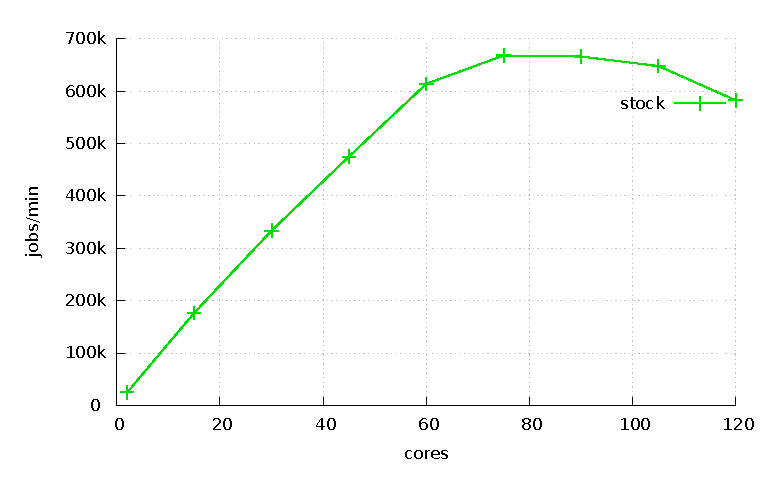
\includegraphics[scale=0.8]{aim7_default}
\end{frame}

\begin{frame}{Performance Scalability}
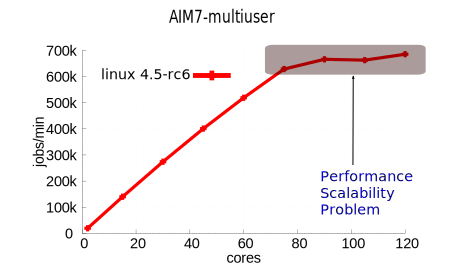
\includegraphics[scale=0.8]{aim7_default_2}
\end{frame}

\begin{frame}{Performance Scalability}
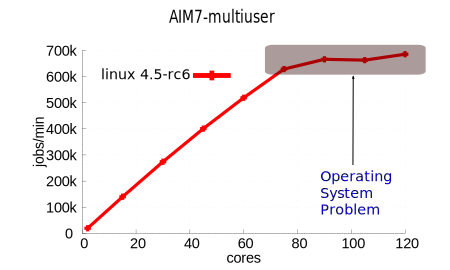
\includegraphics[scale=0.8]{aim7_default_3}
\end{frame}


\begin{frame}{OS Kernel Scalability}
    \begin{itemize}[<+-| alert@+>]
    \item OS kernel scalability is an important part for the whole the system
    parallelism.
    \item If the kernel does not scale, applications will not scale.
    \end{itemize}
\end{frame}


\begin{frame}{AIM7 Scalability}
%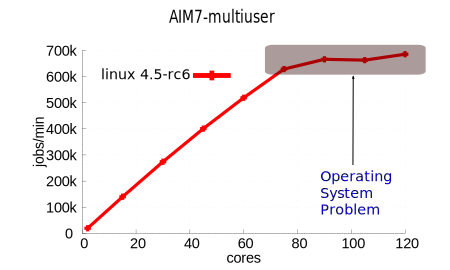
\includegraphics[scale=0.8]{aim7_default_3}
\end{frame}


\begin{frame}{Lock Contention Problem}

\end{frame}


\begin{frame}{Update Serialization}

\end{frame}



\begin{frame}{OS Kernel Scalability Histroy}
\end{frame}


\begin{frame}{OS Kernel Scalability Histroy}
\end{frame}


\begin{frame}{OS Kernel Scalability Histroy}
\end{frame}


\begin{frame}{OS Kernel Scalability Histroy}
\end{frame}


\begin{frame}{OS Kernel Scalability Histroy}
\end{frame}


\begin{frame}{High update rate Data Structuer}
\end{frame}



\begin{frame}{Update-heavy Data structure}
\end{frame}



\begin{frame}{Update-heavy Data structure}
\end{frame}

\begin{frame}{Non-blocking Data Structure}
\end{frame}


\begin{frame}{Non-blocking Data Structure}
\end{frame}


\begin{frame}{Non-blocking Data Structure}
\end{frame}


\begin{frame}{Non-blocking Data Structure}
\end{frame}


\begin{frame}{Cache communication bottlenect}
\end{frame}


\begin{frame}{Cache communication bottlenect}
\end{frame}


\begin{frame}{Cache communication bottlenect}
\end{frame}


\begin{frame}{Cache communication bottlenect}
\end{frame}

\begin{frame}{Cache communication bottlenect}
\end{frame}



\begin{frame}{Approach: Log-based Concurrent Update}
\end{frame}


\begin{frame}{Approach: Log-based Concurrent Update}
\end{frame}


\begin{frame}{Approach: Log-based Concurrent Update}
\end{frame}


\begin{frame}{Advantages of eliminating time-stamp counters}
\end{frame}


\begin{frame}{Contributions}
	\begin{itemize}
	\item Background of research 
	\item Our new method and Evaluation
	\item Future plans and Summary
	\end{itemize}
\end{frame}


\begin{frame}{Outline}
	\begin{itemize}
	\item Design
	\begin{itemize}
	\item Approach
	\item Example 
	\end{itemize}
	\item Applying the Linux kernel
	\item Implementation
	\item Evaluation
	\end{itemize}
\end{frame}


\begin{frame}{Design}
\end{frame}



\begin{frame}{Why the OpLog needs the time-stamp counter?}
\end{frame}



\begin{frame}{Log Example}
\end{frame}




\begin{frame}{Update-side removing}
\end{frame}


\begin{frame}{Garbage log}
\end{frame}


\begin{frame}{Reusing logs}
\end{frame}


\begin{frame}{Approach}
\end{frame}


\begin{frame}{Example}
\end{frame}


\begin{frame}{Example}
\pgfdeclareimage[width=\paperwidth]{ldu}{.//slides/ldu}
\begin{textblock}{1}(0,0)
\pgfuseimage<+->{ldu}
\end{textblock}
\end{frame}

\begin{frame}{Example}
\end{frame}

\begin{frame}{Example}
\end{frame}

\begin{frame}{Example}
\end{frame}

\begin{frame}{Example}
\end{frame}

\begin{frame}{Example}
\end{frame}

\begin{frame}{Example}
\end{frame}

\begin{frame}{Example}
\end{frame}

\begin{frame}{Applying the Linux kernel}
\end{frame}



\begin{frame}{anonymous reverse mapping}
\end{frame}


\begin{frame}{anonymous reverse mapping}
\end{frame}


\begin{frame}{file mapping}
\end{frame}


\begin{frame}{file mapping}
\end{frame}



\begin{frame}{Evaluation}
\end{frame}


\begin{frame}{Non-blocking algorithm - Harris linked list}
\end{frame}

\begin{frame}{Test-bed}
\end{frame}


\begin{frame}{Test-bed}
\end{frame}


\begin{frame}{AIM7}
\end{frame}



\begin{frame}{AIM7 - CPU utilization}
\end{frame}

\begin{frame}{EXIM}
\end{frame}


\begin{frame}{EXIM - CPU utilization}
\end{frame}


\begin{frame}{Lmbench}
\end{frame}


\begin{frame}{Lmbench - CPU utilization}
\end{frame}



\begin{frame}{Update ratio}
\end{frame}


\begin{frame}{Related work}

\end{frame}


\begin{frame}{Papers}

\end{frame}


\begin{frame}{Conclusion}
	\begin{itemize}
	\item Background of research 
	\item LDU method and Evaluation
	\item Future plans and Summary
	\end{itemize}
\end{frame}


\begin{frame}{Conclusion}
    \begin{itemize}
    \item Background of research 
    \item LDU method and Evaluation
    \item Future plans and Summary
    \item \text{https://github.com/KMU-embedded/scalablelinux}
    \end{itemize}
\end{frame}


\end{document}
